% Set Beamer class
%\documentclass{beamer} % <---- with pauses and transitions
\documentclass[handout]{beamer} %<--- flat presentation


% Set theme and color scheme, see [1].
\usetheme{Warsaw}
\usecolortheme{wolverine}

% Beamer Transparence level
\setbeamercovered{transparent=15}

% My Packages
\usepackage{lipsum}
\usepackage{multicol}

% Set basica parameters
\title[Tutorial class]{My Presentation}
\subtitle{Learning to use the Beamer class}
\author[D{\'i}az, Gonz{\'a}les]
{
    Manuel A. D{\'i}az\inst{1} 
    \and 
    Juan C. Gonz{\'a}les\inst{2}
}
\institute[TECNM]
{
    \inst{1}
    {\'E}cole Sup{\'e}riere de M{\'e}canique et d'A{\'e}rotechnique\\
    Poitiers, France
    \and
    \inst{2}
    Universidad Ju{\'a}rez Aut{\'o}noma de Tabasco \\
    Villahermosa, Tabasco, Mexico
}
\date{\today}
\logo{\includegraphics[height=1cm]{figures/TECNM.png}}

% Beging document
\begin{document}

\begin{frame}
    \titlepage
\end{frame}

\begin{frame}{Outline}
    \tableofcontents
\end{frame}

%%%%%%%%%%%%%%%%%%%%%%%%%
\section{A basic frames}
%%%%%%%%%%%%%%%%%%%%%%%%%

\subsection{Frame mechanics}
\begin{frame}[t]{Introduction}
    \begin{figure}
        
\includegraphics[width=0.5\textwidth]{figures/TeXlion.jpg}
        \caption{Leo}
    \end{figure}
    Welcome TeXnicians !
\end{frame}

\subsection{A table in latex}
\begin{frame}[c]
    \begin{table}
    \begin{tabular}{ l | c | c | c | c }
    Competitor Name & Swim & Cycle & Run & Total \\
    \hline \hline
    John T & 13:04 & 24:15 & 18:34 & 55:53 \\ 
    Norman P & 8:00 & 22:45 & 23:02 & 53:47\\
    Alex K & 14:00 & 28:00 & n/a & n/a\\
    Sarah H & 9:22 & 21:10 & 24:03 & 54:35 
    \end{tabular}
    \caption{Triathlon results}
    \end{table}
\end{frame}

\subsection{Lists \& enumerated lists}
\begin{frame}[t]{Listing things}
    \begin{itemize}
        \item this is item 1
        \begin{enumerate}
            \item this is subitem 1
            \item \underline{this is subitem 2}
            \item \alert{this is subitem 3}
        \end{enumerate} 
        \pause
        \item this is item 2
        \begin{enumerate}[(i)]
            \item {\color{red} this is subitem 1}
            \item \bf{this is subitem 2}
        \end{enumerate} 
        \item this is item 3
        \pause
        \begin{enumerate}[(I)]
            \item {\color{green} this is subitem 1}
            \item \it{this is subitem 2}
        \end{enumerate} 
    \end{itemize}
    %
\end{frame}

\subsection{Highlighting text}

\subsection{Block definitions}
\begin{frame}{A block definitions}
    %
    \begin{block}{The advection equation:}
        \begin{equation}
            \partial_{t} u + \nabla\cdot f(u) = 0,
        \end{equation}
    \end{block}
    %
    \pause
    \begin{alertblock}{The heat equation:}
        \begin{equation}
            \partial_{t} u = \nabla^2 u + \sigma.
        \end{equation}
    \end{alertblock}
    %
    \pause
    adding the above equations yields:
    %
    \pause
    \begin{exampleblock}{The advection-diffusion equation:}
        \begin{equation}
            \partial_{t} u + \nabla\cdot f(u) = \nabla^2 u + \sigma.
        \end{equation}
    \end{exampleblock}
    %
\end{frame}

\subsection{Workin with columns}
\begin{frame}[t]{Working in two-columns}
    \begin{columns}[onlytextwidth]
        \column{0.5\textwidth}
        \small{\lipsum[4]}
        \column{0.5\textwidth}
        \vspace{-1cm}
        \begin{figure}
            \only<1>{
            \caption{Subsonic Monopole}
            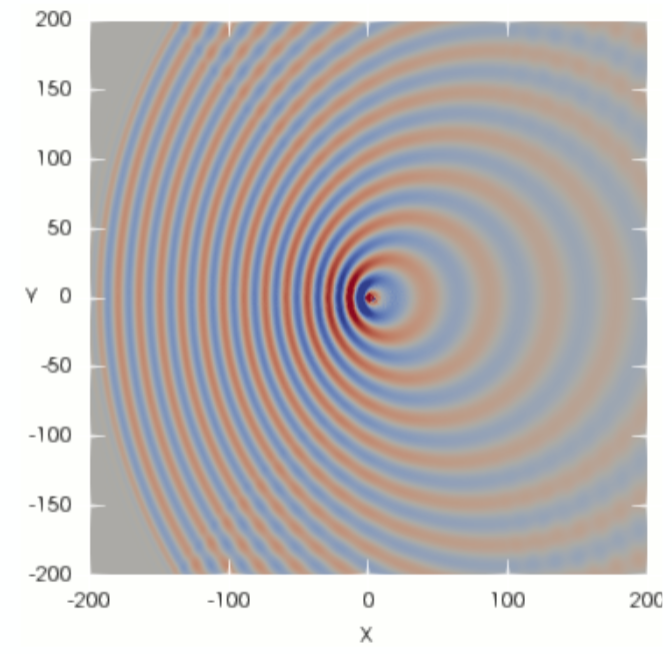
\includegraphics[width=0.9\textwidth]{figures/Mach03.png}
            }
            \only<2>{
            \caption{Supersonic Monopole}
            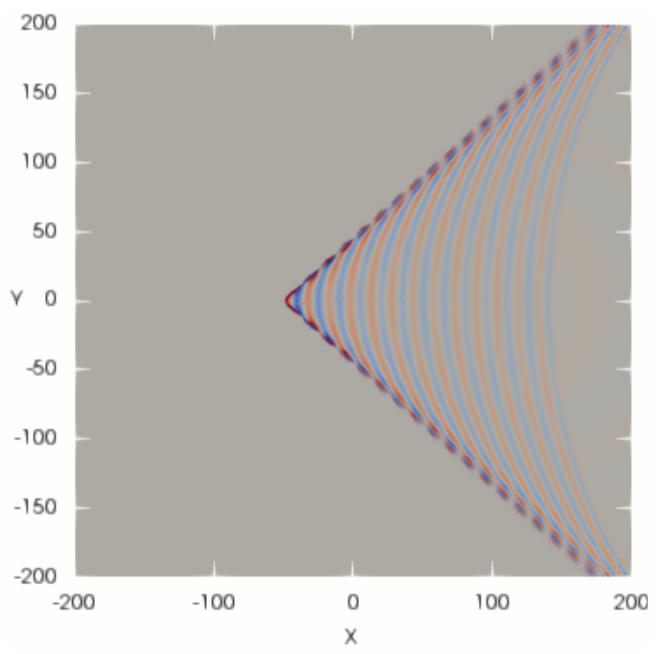
\includegraphics[width=0.9\textwidth]{figures/Mach12.png}
            }
        \end{figure}
    \end{columns}
\end{frame}

\begin{frame}[t]{List in multiple columns}
    \begin{enumerate}
        \begin{multicols}{3}
        \item $y = x$
        \item $y = |x|$
        \item $y = x^2$
        \item $y = x^3$
        \item $y = x^b$
        \onslide<2->{
        \item $y = \sqrt{x}$
        \item $y = \sqrt[3]{x}$
        \item $y = \frac{1}{x}$
        \item $y = \ln x$
        \item $y = \frac{1}{1+e^{-x}}$
        }
        \onslide<3->{
        \item $y = \sin x$
        \item $y = \cos x$
        \item $y = \tan x$
        \item $y = 2^x$
        \item $y = e^x$
        }
        \end{multicols}
    \end{enumerate}
\end{frame}

\subsection{Frame breaks}
\begin{frame}[t,allowframebreaks]{References}
    \small{\lipsum[1-2]}
\end{frame}

\begin{frame}%[standout]
    %\flushleft
    Any Questions?
\end{frame}

\end{document}